\documentclass[11pt,preprint]{elsarticle}

\usepackage{lmodern}
%%%% My spacing
\usepackage{setspace}
\setstretch{1.2}
\DeclareMathSizes{12}{14}{10}{10}

% Wrap around which gives all figures included the [H] command, or places it "here". This can be tedious to code in Rmarkdown.
\usepackage{float}
\let\origfigure\figure
\let\endorigfigure\endfigure
\renewenvironment{figure}[1][2] {
    \expandafter\origfigure\expandafter[H]
} {
    \endorigfigure
}

\let\origtable\table
\let\endorigtable\endtable
\renewenvironment{table}[1][2] {
    \expandafter\origtable\expandafter[H]
} {
    \endorigtable
}


\usepackage{ifxetex,ifluatex}
\usepackage{fixltx2e} % provides \textsubscript
\ifnum 0\ifxetex 1\fi\ifluatex 1\fi=0 % if pdftex
  \usepackage[T1]{fontenc}
  \usepackage[utf8]{inputenc}
\else % if luatex or xelatex
  \ifxetex
    \usepackage{mathspec}
    \usepackage{xltxtra,xunicode}
  \else
    \usepackage{fontspec}
  \fi
  \defaultfontfeatures{Mapping=tex-text,Scale=MatchLowercase}
  \newcommand{\euro}{€}
\fi

\usepackage{amssymb, amsmath, amsthm, amsfonts}

\def\bibsection{\section*{References}} %%% Make "References" appear before bibliography


\usepackage[numbers]{natbib}

\usepackage{longtable}
\usepackage[margin=2.3cm,bottom=2cm,top=2.5cm, includefoot]{geometry}
\usepackage{fancyhdr}
\usepackage[bottom, hang, flushmargin]{footmisc}
\usepackage{graphicx}
\numberwithin{equation}{section}
\numberwithin{figure}{section}
\numberwithin{table}{section}
\setlength{\parindent}{0cm}
\setlength{\parskip}{1.3ex plus 0.5ex minus 0.3ex}
\usepackage{textcomp}
\renewcommand{\headrulewidth}{0.2pt}
\renewcommand{\footrulewidth}{0.3pt}

\usepackage{array}
\newcolumntype{x}[1]{>{\centering\arraybackslash\hspace{0pt}}p{#1}}

%%%%  Remove the "preprint submitted to" part. Don't worry about this either, it just looks better without it:
\makeatletter
\def\ps@pprintTitle{%
  \let\@oddhead\@empty
  \let\@evenhead\@empty
  \let\@oddfoot\@empty
  \let\@evenfoot\@oddfoot
}
\makeatother

 \def\tightlist{} % This allows for subbullets!

\usepackage{hyperref}
\hypersetup{breaklinks=true,
            bookmarks=true,
            colorlinks=true,
            citecolor=blue,
            urlcolor=blue,
            linkcolor=blue,
            pdfborder={0 0 0}}


% The following packages allow huxtable to work:
\usepackage{siunitx}
\usepackage{multirow}
\usepackage{hhline}
\usepackage{calc}
\usepackage{tabularx}
\usepackage{booktabs}
\usepackage{caption}


\newenvironment{columns}[1][]{}{}

\newenvironment{column}[1]{\begin{minipage}{#1}\ignorespaces}{%
\end{minipage}
\ifhmode\unskip\fi
\aftergroup\useignorespacesandallpars}

\def\useignorespacesandallpars#1\ignorespaces\fi{%
#1\fi\ignorespacesandallpars}

\makeatletter
\def\ignorespacesandallpars{%
  \@ifnextchar\par
    {\expandafter\ignorespacesandallpars\@gobble}%
    {}%
}
\makeatother


% definitions for citeproc citations
\NewDocumentCommand\citeproctext{}{}
\NewDocumentCommand\citeproc{mm}{%
\href{\#cite.\detokenize{#1}}{#2}\nocite{#1}}

\makeatletter
% allow citations to break across lines
\let\@cite@ofmt\@firstofone
% avoid brackets around text for \cite:
\def\@biblabel#1{}
\def\@cite#1#2{{#1\if@tempswa , #2\fi}}
\makeatother
\newlength{\cslhangindent}
\setlength{\cslhangindent}{1.5em}
\newlength{\csllabelwidth}
\setlength{\csllabelwidth}{3em}
\newenvironment{CSLReferences}[2] % #1 hanging-indent, #2 entry-spacing
{\begin{list}{}{%
	\setlength{\itemindent}{0pt}
	\setlength{\leftmargin}{0pt}
	\setlength{\parsep}{0pt}
	% turn on hanging indent if param 1 is 1
	\ifodd #1
	\setlength{\leftmargin}{\cslhangindent}
	\setlength{\itemindent}{-1\cslhangindent}
	\fi
	% set entry spacing
	\setlength{\itemsep}{#2\baselineskip}}}
{\end{list}}

\usepackage{calc}
\newcommand{\CSLBlock}[1]{\hfill\break\parbox[t]{\linewidth}{\strut\ignorespaces#1\strut}}
\newcommand{\CSLLeftMargin}[1]{\parbox[t]{\csllabelwidth}{\strut#1\strut}}
\newcommand{\CSLRightInline}[1]{\parbox[t]{\linewidth - \csllabelwidth}{\strut#1\strut}}
\newcommand{\CSLIndent}[1]{\hspace{\cslhangindent}#1}


\urlstyle{same}  % don't use monospace font for urls
\setlength{\parindent}{0pt}
\setlength{\parskip}{6pt plus 2pt minus 1pt}
\setlength{\emergencystretch}{3em}  % prevent overfull lines
\setcounter{secnumdepth}{5}

%%% Use protect on footnotes to avoid problems with footnotes in titles
\let\rmarkdownfootnote\footnote%
\def\footnote{\protect\rmarkdownfootnote}
\IfFileExists{upquote.sty}{\usepackage{upquote}}{}

%%% Include extra packages specified by user
\usepackage{booktabs}
\usepackage{longtable}
\usepackage{array}
\usepackage{multirow}
\usepackage{wrapfig}
\usepackage{float}
\usepackage{colortbl}
\usepackage{pdflscape}
\usepackage{tabu}
\usepackage{threeparttable}
\usepackage{threeparttablex}
\usepackage[normalem]{ulem}
\usepackage{makecell}
\usepackage{xcolor}

%%% Hard setting column skips for reports - this ensures greater consistency and control over the length settings in the document.
%% page layout
%% paragraphs
\setlength{\baselineskip}{12pt plus 0pt minus 0pt}
\setlength{\parskip}{12pt plus 0pt minus 0pt}
\setlength{\parindent}{0pt plus 0pt minus 0pt}
%% floats
\setlength{\floatsep}{12pt plus 0 pt minus 0pt}
\setlength{\textfloatsep}{20pt plus 0pt minus 0pt}
\setlength{\intextsep}{14pt plus 0pt minus 0pt}
\setlength{\dbltextfloatsep}{20pt plus 0pt minus 0pt}
\setlength{\dblfloatsep}{14pt plus 0pt minus 0pt}
%% maths
\setlength{\abovedisplayskip}{12pt plus 0pt minus 0pt}
\setlength{\belowdisplayskip}{12pt plus 0pt minus 0pt}
%% lists
\setlength{\topsep}{10pt plus 0pt minus 0pt}
\setlength{\partopsep}{3pt plus 0pt minus 0pt}
\setlength{\itemsep}{5pt plus 0pt minus 0pt}
\setlength{\labelsep}{8mm plus 0mm minus 0mm}
\setlength{\parsep}{\the\parskip}
\setlength{\listparindent}{\the\parindent}
%% verbatim
\setlength{\fboxsep}{5pt plus 0pt minus 0pt}



\begin{document}



\begin{frontmatter}  %

\title{Question 4: Billionaires}

% Set to FALSE if wanting to remove title (for submission)




\author[Add1]{Matthew Thompson}
\ead{22892435@sun.ac.za}





\address[Add1]{Department of Economics, Stellenbosch University}



\vspace{1cm}





\vspace{0.5cm}

\end{frontmatter}

\setcounter{footnote}{0}



%________________________
% Header and Footers
%%%%%%%%%%%%%%%%%%%%%%%%%%%%%%%%%
\pagestyle{fancy}
\chead{}
\rhead{}
\lfoot{}
\rfoot{\footnotesize Page \thepage}
\lhead{}
%\rfoot{\footnotesize Page \thepage } % "e.g. Page 2"
\cfoot{}

%\setlength\headheight{30pt}
%%%%%%%%%%%%%%%%%%%%%%%%%%%%%%%%%
%________________________

\headsep 35pt % So that header does not go over title




\section{\texorpdfstring{Introduction
\label{Introduction}}{Introduction }}\label{introduction}

To tackle this problem, we investigate a few relationships found in the
data. The first one we'd like to examine is the claim that the US has
more new billionaires who came from entrepreneurial success vs in other
developed and emerging economies where there tends to be more inherited
wealth.\\
Thereafter, we perform a sectoral analysis to see if the software sector
is indeed the host of most of the new billionaires when compared to
other sectors.\\
Analysis finds both claims to be invalid.

\section{Entrepreneurial spirit in US vs
Others}\label{entrepreneurial-spirit-in-us-vs-others}

We start by examining the United States billionaire landscape on its
own, checking to see how many of the billionaires came from
entrepreneurship and how many came from inherited wealth.\\
First want to extract US billionaires only.

After that, want to compare their sources of wealth and how it changed
over the 3 time periods. For each period, want to calculate the
proportion of wealth that was inherited and that which was not
inherited.

We use a simple pie chart to display the change in proportion of those
who inherited wealth over the 3 time periods.

\begin{figure}[H]

{\centering 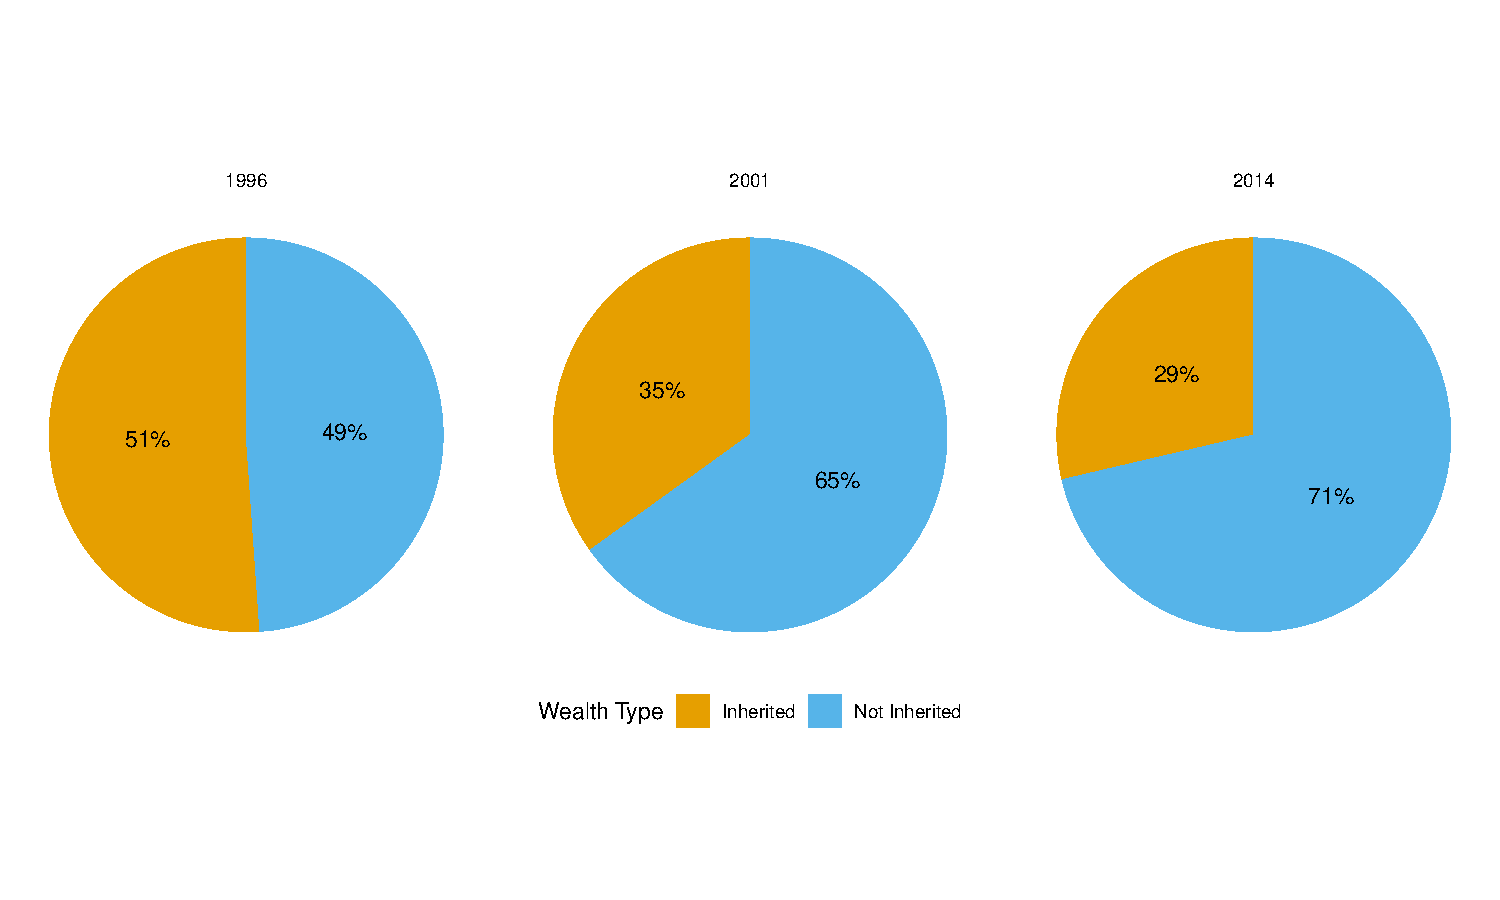
\includegraphics[width=0.8\linewidth]{./output/fig1} 

}

\caption{Pie chart showing proportions of US billionaires that had inherited vs those that did not inherit their wealth \label{Fig1}}\label{fig:unnamed-chunk-2}
\end{figure}

The following table also shows how even though the proportion of
inherited wealth has decreased relative to non-inherited sources, the
number of billionaires who have inherited their wealth has increased.

\begin{table}
\centering
\caption{\label{tab:US inheritance table}Table showing the US inheritance statistics \label{tab1}}
\centering
\begin{tabular}[t]{c|c|c}
\hline
Year & No. of billionaires who inherited their wealth & No. of billionaires who have not inherited their wealth\\
\hline
1996 & 69 & 66\\
\hline
2001 & 94 & 175\\
\hline
2014 & 143 & 356\\
\hline
\end{tabular}
\end{table}

This leads us to investigate what entrepreneurial spirit and inherited
wealth looks like in countries outside of the United States.\\
We begin again by extracting all the billionaires from outside of the
US.

Then we obtain the proportion of this group that have inherited their
wealth vs those that have not.

\begin{figure}[H]

{\centering 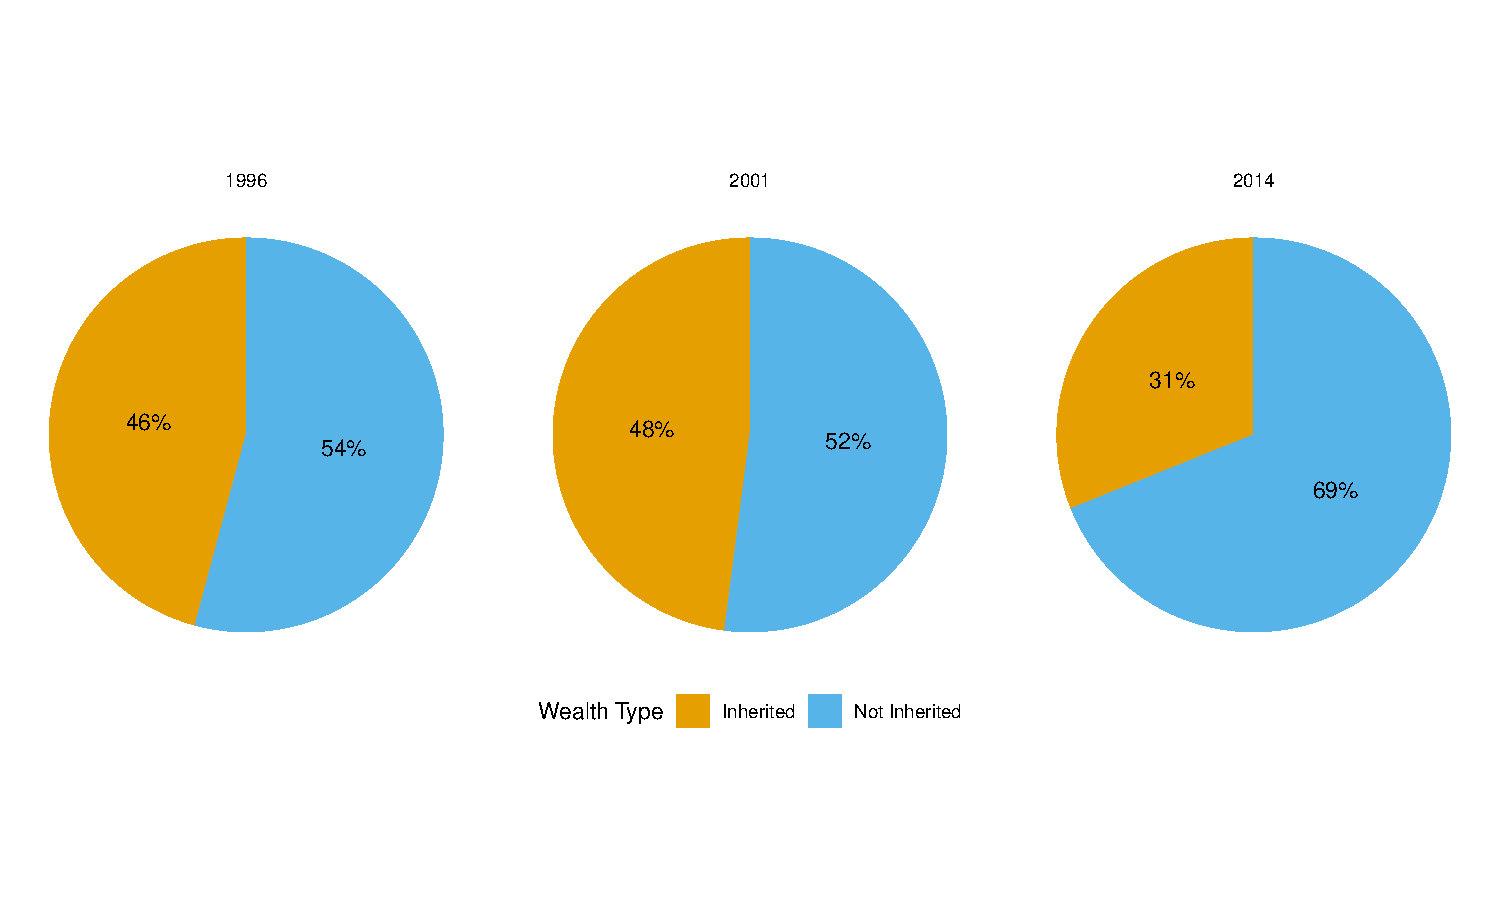
\includegraphics[width=0.8\linewidth]{./output/fig2} 

}

\caption{Pie chart showing proportions of those outside of the US billionaires that had inherited vs those that did not inherit their wealth \label{Fig2}}\label{fig:unnamed-chunk-3}
\end{figure}

\begin{table}
\centering
\caption{\label{tab:Outside US inheritance table}Table showing Outside of the US inheritance statistics \label{tab2}}
\centering
\begin{tabular}[t]{c|c|c}
\hline
Year & No. of billionaires who inherited their wealth & No. of billionaires who have not inherited their wealth\\
\hline
1996 & 132 & 156\\
\hline
2001 & 129 & 140\\
\hline
2014 & 359 & 795\\
\hline
\end{tabular}
\end{table}

Figure \ref{Fig2} shows us that while there was a decrease in the
proportion of those who obtained their wealth from non-inheritance over
1996-2001, a large increase in this proportion occurred over 2001-2014.
Note also how in each period the proportion of those who made their
wealth from non-inheritance is greater than half of the population of
billionaires outside of the US. This contradicts the statement saying
that outside the US houses billionaires who've mostly sourced their
wealth from inheritance.

Tables \ref{tab1} and \ref{tab2} show how even though the US has a
slightly higher proportion over time of those billionaires who had not
inherited their wealth which had increased over the time periods, those
from outside of the US also experienced a decrease in proportion of the
number of wealthy coming from inheritance.

A simple calculation shows that the growth rate for those who have
inherited wealth in the US is 36.2\% for 2001 and 52.1\% over 2014, and
165.2\% and 103.4\% for those who have not inherited wealth. These same
rates for those outside of the US are -2.3\% for 2001 and 178.3\%, and
-10.3\% and 467.9\%. What these figures show is that those from outside
of the US have experienced the largest growth rate in the number of new
billionaires who have not come from inherited wealth. This contradicts
the first statement, showing that there may be a stronger
entrepreneurial spirit displayed by those from outside of the US in more
recent years, seen with the higher growth rate when compared to that of
the US over 2001-2014.

\section{Sector analysis}\label{sector-analysis}

This section lays out the analysis of the second statement that most
new-made millionaires are in software, compared to consumer services
type industries of the 90s.

Here I created a plot showcasing the top 10 billionaire sectors while
using number of billionaires in software as a measuring device.

\begin{figure}[H]

{\centering 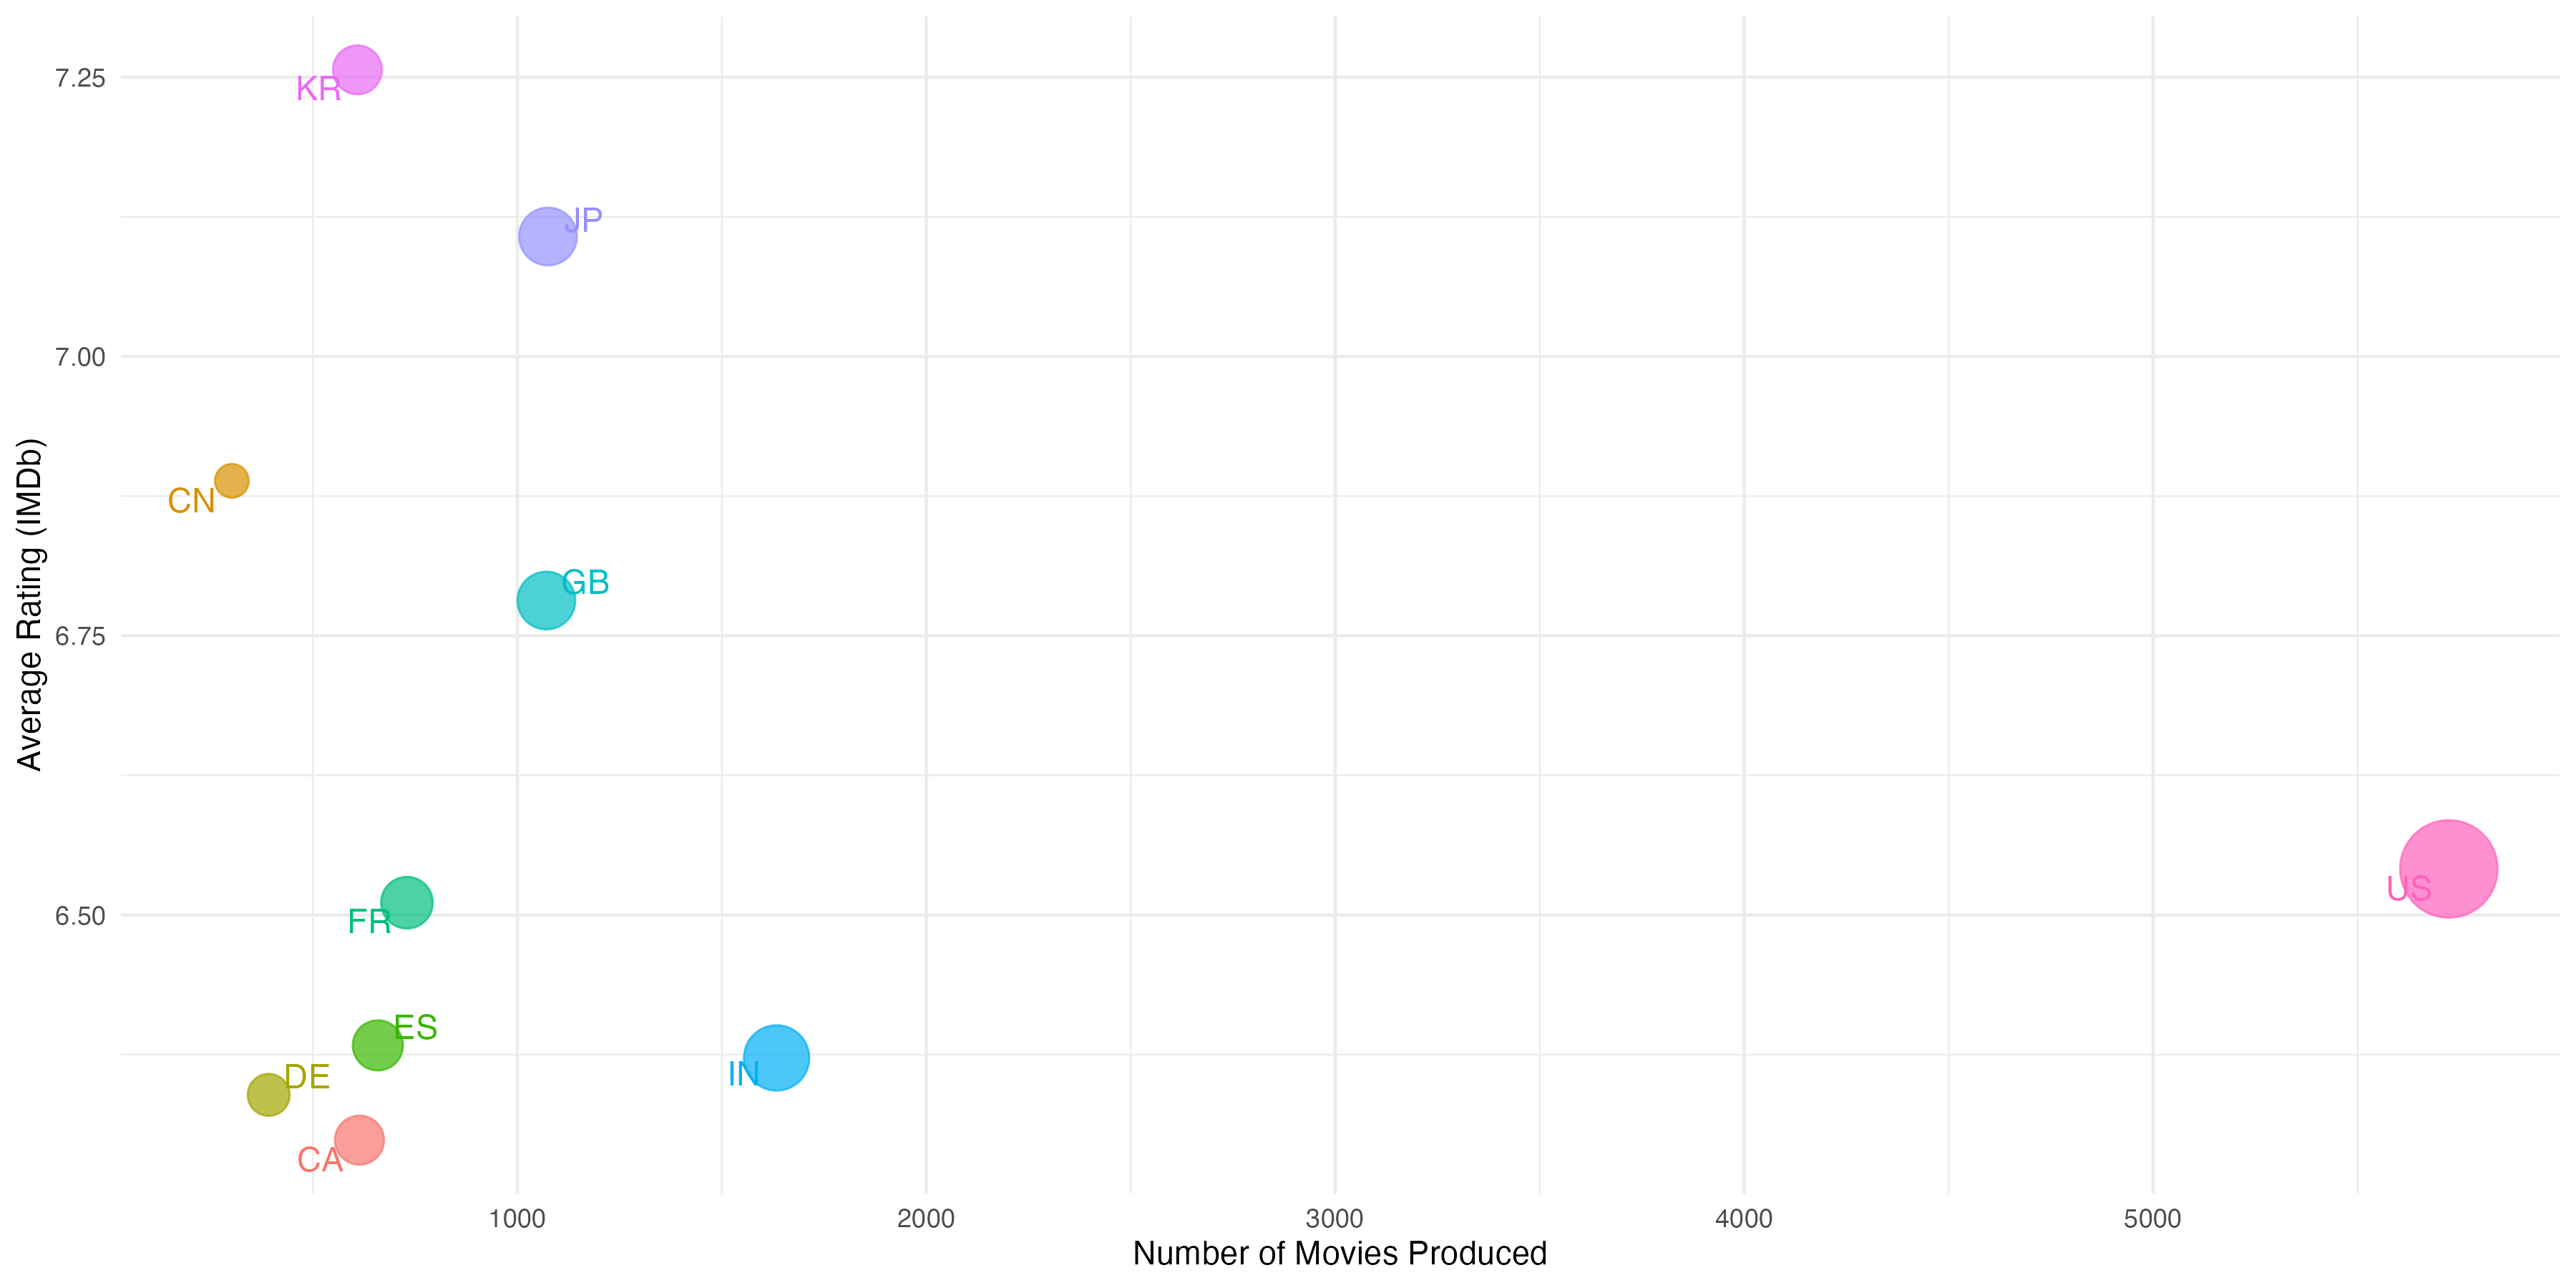
\includegraphics[width=0.8\linewidth]{./output/fig3} 

}

\caption{Column plots showing the top 10 billionaire sectors over the 3 periods, using the number of software billionaires as a benchmark in each \label{Fig3}}\label{fig:unnamed-chunk-5}
\end{figure}

Figure \ref{Fig3} shows that the second statement is also not valid.
Clearly, the number of billonaires in the software sector are lagging
behind many sectors such as real estate, retail, construction, media,
banking, pharmaceuticals and hedge funds.\\
To evaluate the second part of this statement we include GDP per country
in the analysis. This entails using a simple linear regression to model
if coming from a richer country increases or decreases the probability
of the billionaire being part of the software sector.

\begin{table}
\centering
\caption{\label{tab:unnamed-chunk-6}Table showing results of regression of log of GDP on the probability of being in the software sector \label{tab3}}
\centering
\begin{tabular}[t]{l|r|r|r|r}
\hline
Variable & Coefficient & Std. Error & Statistic & p-value\\
\hline
(Intercept) & -7.223 & 4.763 & -1.516 & 0.130\\
\hline
ln\_gdp & 0.006 & 0.003 & 1.909 & 0.057\\
\hline
year & 0.004 & 0.002 & 1.481 & 0.139\\
\hline
\end{tabular}
\end{table}

Table \ref{tab3} also shows contradictory information to the second
statement made. It shows that there is a very small and positive
insignificant linear relationship between GDP and the probability of a
billionaire being in the software sector, after including for time
controls.

\section{Conclusion}\label{conclusion}

Through the various plots and tables provided, I have shown evidence
that both claims made are unfounded.\\
Firstly, it is not only in the US that less billionaires are having
their wealth sourced through inheritances. Billionaires of
non-inheritance from around the world experienced a higher growth rate
than that of those from the US in recent years.\\
Secondly, the software sector lags behind other sectors when it comes to
creating new billionaires in recent times.

\bibliography{Tex/ref}





\end{document}
